\subsection{Design Overview}
We split our software into three parts in series. The first part is image preprocessing, in which we use deep learning methods discussed in the previous section to automatically generate annotation hints for the image. The image and hints are then shown to the user through our GUI interface. Built upon Qt framework, the GUI will provide a clear interface and convenient functions so that human annotator can easily annotate the image with the help of hints. The final annotation information will be generated in JSON format. Then the annotation process for one image is completed and this process will repeat for every image to be annotated. The process is shown as a flow chart in Fig.\ref{fig:FlowChart}.


\begin{figure}[h!]
  \centering 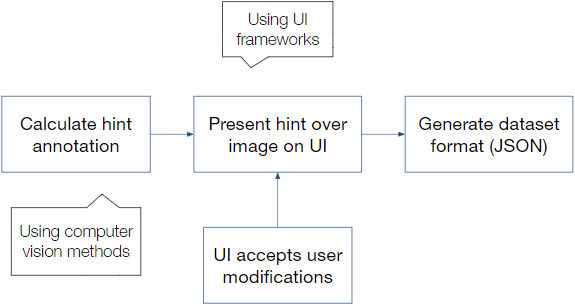
\includegraphics[width=\linewidth]{flow_chart.png}
  \caption{Final Design Flow Chart}
  \label{fig:FlowChart}
\end{figure}


\subsection{Engineering Design Analysis}
\subsubsection{Image Processing}
In this part, knowledge in deep learning and machine learning is required. Basic knowledge on the concept of modern computer vision techniques, including computer vision tasks and their corresponding models, is very helpful. The specific parameters involved in this part are the hyperparameters and parameters in deep learning models. To determine the parameters, deep learning framework \textit{Keras} is used to train those variables.

\begin{enumerate}
    \item \textbf{Object detection} In object detection, we choose a state-of-the-art model: You Only Look Once(YOLO)\cite{Redmon2018YOLOv3}. It can detect the 20 Pascal object classes: person, cow, dog, horse, sheep, bicycle, boat, bus, car, motorbike, train, bottle, chair, dining table, potted, plant, sofa, tv monitor. 
    
%     A single convolutional network simultaneously predicts multiple bounding boxes and class probabilities for
% those boxes. YOLO trains on full images and directly optimizes detection performance.



The reason for choosing the threshold, i.e. confidence level as $60\%$ is due to our requirement to reduce false positives. We have done experiments over a number of parameters on the given dataset to make sure that all objects in our data are detected without creating too many false positives. The criteria we used to help with the decision

$$
\frac{\#\text{false positive}}{\#\text{total objects}} < 0.1,\ \text{and} \ \frac{\#\text{recall}}{\#\text{total objects}}> 0.5
$$
There are also several other parameters for tuning while training: 

\begin{itemize}
    \item Momentum: We chose the default as 0.9 and also tested others. The weights of a neural network are updated based on a small batch of images and not the entire dataset in order to make our training faster. Because of this reason, the weight updates fluctuate quite a bit. That is why a parameter momentum is used to penalize large weight changes between iterations. 
    
    \item Decay: A YOLOv3 has millions of weights and therefore they can easily overfit any training data. Overfitting simply means it will do very well on training data and poorly on test data. One of the ways to mitigate this problem is to penalize large value for weights. The parameter decay controls this penalty term. We chose the default \texttt{decay = 0.0005} and also tested other values, which proves that the default gives best performance. 
    \item Data augmentation parameters: \texttt{angle=0, saturation=1.5, exposure=1.5, hue=.1} The angle parameter in the configuration file allows us to randomly rotate the image. And saturation, exposure and hue allow us to change the image lightening conditions for training. Since our test data given by HJ Drive is taken in cloudy conditions, we tuned the saturation, exposure and hue a little bit to make the training data more alike to our test-data. We did a grid search to find that the above parameters show the best accuracy for testing.  
\end{itemize}


\end{enumerate}





\subsubsection{GUI Design}
In this part, the related field is human computer interaction (HCI). Experience in graphical interface and website design is needed. 

\subsection{Design Description}
% \yueying{Software projects are required to explain their projects in sub-function using animations or flow charts if necessary. It should not only be clear what the final design is, but how it can be made, how it will work, and why it will work. List all parts used and their cost. In short, the description should be detailed enough for another team to build the final prototype, using this report as a reference. 
% }

In this part, we introduce the design of each component in the system before delving into some notable design details. At the top level, the labelling system consists of 3 subsystems:
\begin{itemize}
    \item Graphical user interface (GUI): an efficient, interactive user interface, which converts between the information the whole system has or requires and its graphics representations.
    \item Dataset server: a remote program that contains the dataset information and can communicate with the GUI as client.
    \item Deep learning models: models residing on the remote dataset server that for each image, give a reasonably accurate answer to some subtasks of the dataset annotation task.
\end{itemize}

We now discuss each part in greater details, in which how they interact will gradually become clear. Below, \textit{Finite State Machine} (FSM) diagrams are used in the place of the conventional flowcharts to illustrate the functionality of components, due to the state-and-transition nature of GUI systems.

\subsubsection{Graphical user Interface (GUI)}
\label{sec:gui}

Fig. \ref{fig:structure_gui} renders a component breakdown of our GUI subsystem, while the look of some component are displayed in Fig. \ref{fig:look_gui}. In terms of implementation, now we explain several notable details.

\begin{figure}[htbp!]
    \centering
    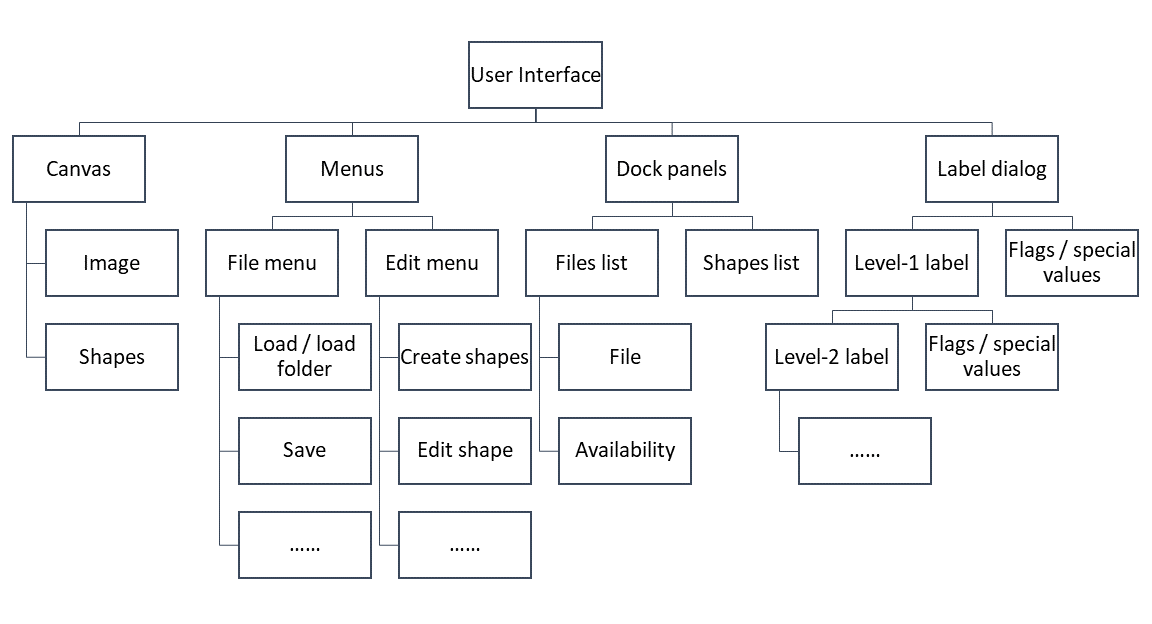
\includegraphics[width=\textwidth]{figures/structure1.png}
    \caption{Component structure of GUI subsystem.}
    \label{fig:structure_gui}
\end{figure}

\begin{figure}[htbp!]
    \centering
    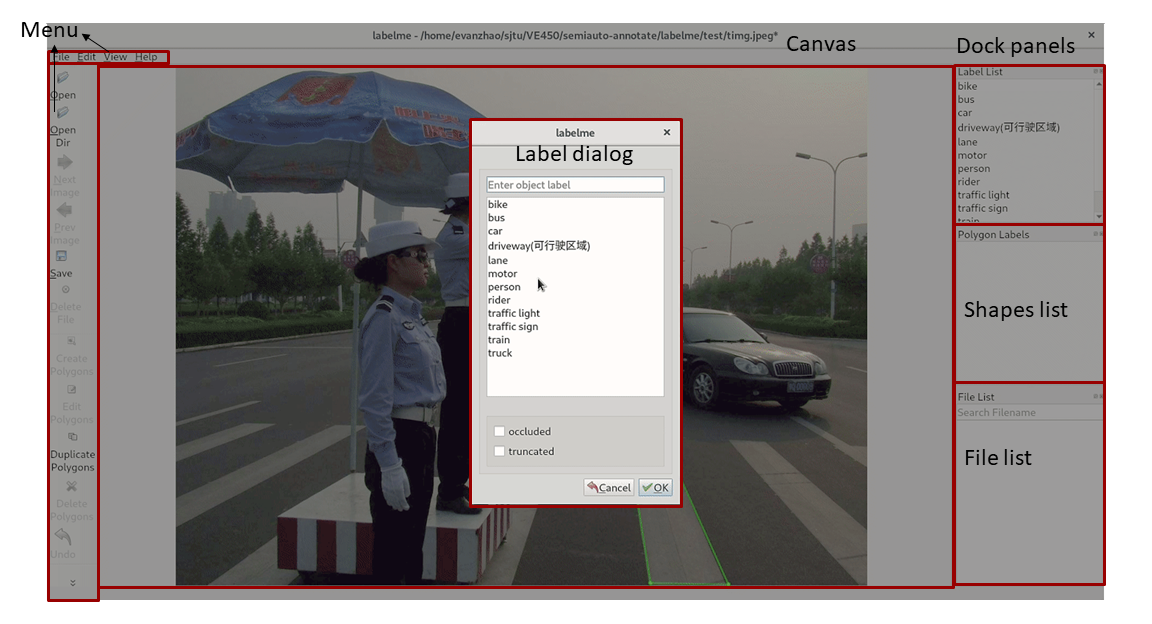
\includegraphics[width=\textwidth]{figures/look.png}
    \caption{Appearance of some GUI components.}
    \label{fig:look_gui}
\end{figure}

\paragraph{Framework} The GUI is implemented under the \texttt{PyQt} framework, a \texttt{Python} binding of the \texttt{C++}-based \texttt{Qt} framework. \texttt{PyQt} provides some \textit{widgets} (GUI components), an abstract model for building custom widgets on, and a signal-event model for processing user inputs. For example, ``files list'' and ``shapes list'' from Fig. \ref{fig:structure_gui} are built-in \texttt{QListWidget}s, while ``canvas'' is a custom widget.

\paragraph{Event processing} The previously mentioned \texttt{PyQt} ``signal-event model'' is a programming scheme, where instead of actively querying the framework for user inputs, each widget register a function for handling such inputs. On certain events' occurrence (such as mouse click), the framework emits a \textit{signal} (such as \texttt{mouseClicked}) and looks for a \textit{slot} (a registered function) to handle it. 

At a high level, the states each component is in, and the signal-events which push the component into another state, make up a finite state machine representation. Here, Fig. \ref{fig:fsm_gui} provides such an FSM representation of our GUI subsystem. While Fig. \ref{fig:structure_gui} displays the \textit{static structure} of GUI, Fig. \ref{fig:fsm_gui} captures the \textit{dynamic behavior} of our GUI subsystem.

In Fig. \ref{fig:fsm_gui}, states are displayed as rectangles; a list of operation the GUI performs when in the state is given under each state. Text in blue is (high-level) events that push the state transition, and text in red is actions that immediately occur upon the event. Due to the complexity of the software, only the most critical states are shown in the diagram.

\begin{figure}[htbp!]
    \centering
    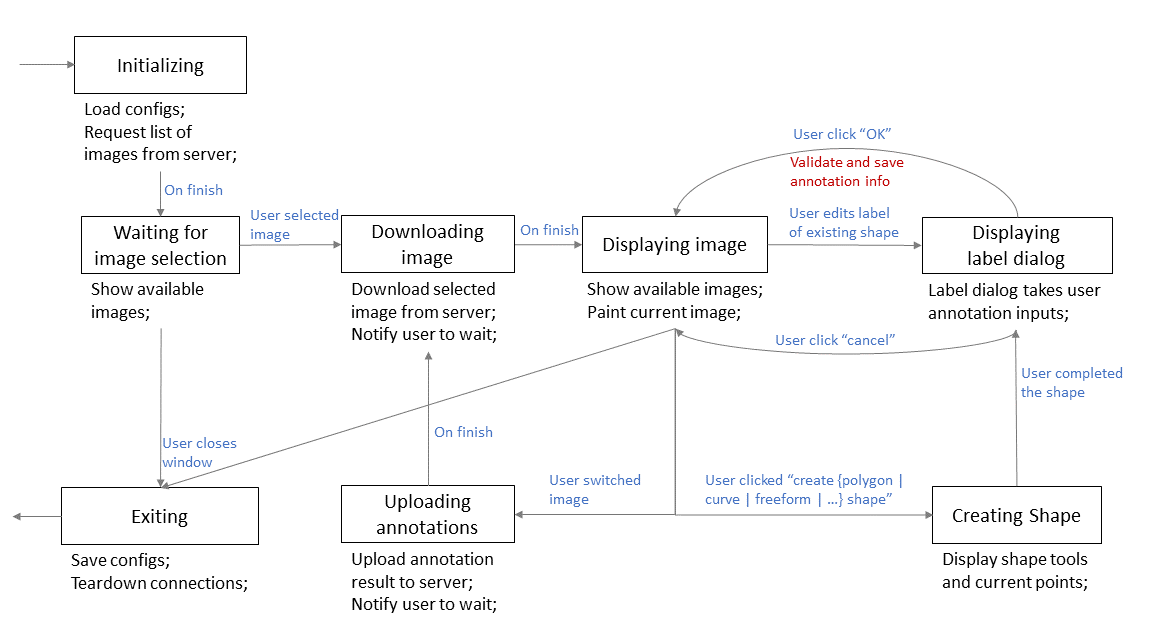
\includegraphics[width=\textwidth]{figures/fsm1.png}
    \caption{FSM representation of GUI subsystem.}
    \label{fig:fsm_gui}
\end{figure}

\subsubsection{Dataset Server}

\begin{figure}
    \centering
    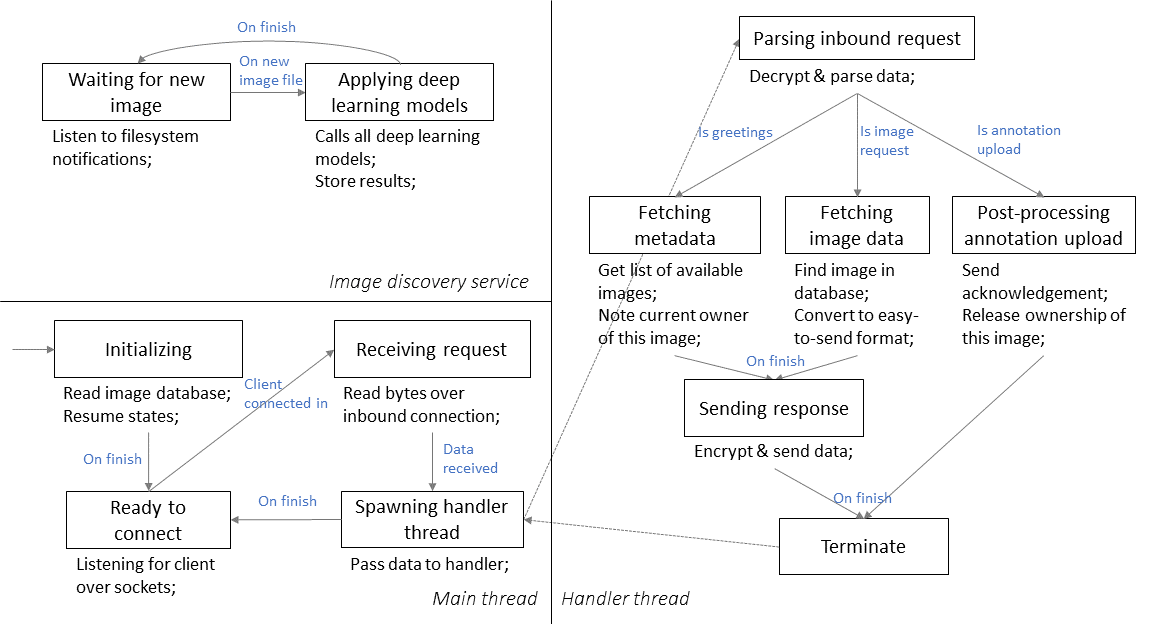
\includegraphics[width=\textwidth]{figures/fsm2.png}
    \caption{FSM representation of dataset server subsystem.}
    \label{fig:fsm_server}
\end{figure}

The behavior of dataset server is given in Fig. \ref{fig:fsm_server}. Notations are the same as used in description of GUI (\S\ref{sec:gui}). Similarly:

\paragraph{Framework} The server is implemented under the \texttt{Flask} framework in Python. \texttt{Flask} provides endpoint-handler logic, where the programmer defines a list of \textit{endpoints}, each with a function which is called when the user accesses that endpoint. (Endpoint is the chain in an URL after the domain name; for example, \url{https://example.com/a/b/c} would have an endpoint of \url{a/b/c}.)

\paragraph{Common Practices of Server Implementation} A naive implementation of server would be a single-threaded one, where the main thread accepts connection, receives data, compute response, send response, return to listening -- leaving the server \textit{suspended} whenever the main thread is busy with a request. To improve the availability of the server, a common practice is, instead, to create a \textit{handler} thread when a client connects in. While creating threads incur overhead, it is almost always negligible in the face of slower operations, such as reading files, communicating data over network, etc.

\paragraph{Interaction between dataset server and GUI client} Fig. \ref{fig:interaction} represents the interaction between server and client by combining their FSMs in the same diagram. 

\begin{figure}
    \centering
    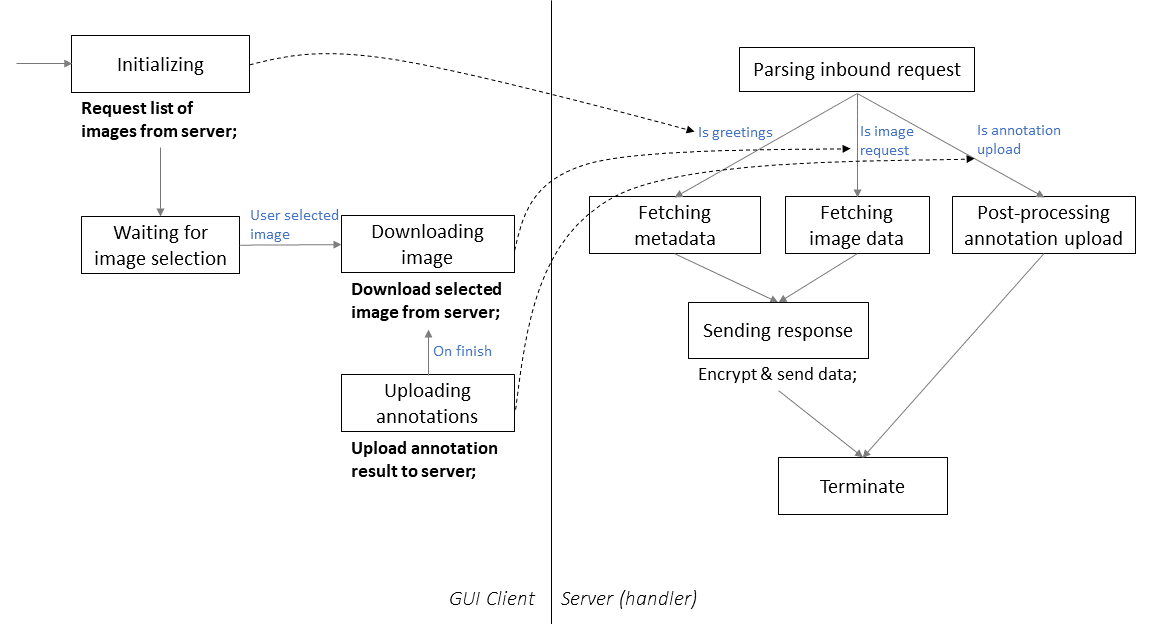
\includegraphics[width=\textwidth]{figures/interaction.png}
    \caption{Interaction between server and clients.}
    \label{fig:interaction}
\end{figure}

\paragraph{Interaction between dataset server and deep learning models} Deep learning models generally reside on the server. As shown in \ref{fig:fsm_server}, the server spawns a \textit{image discovery thread}, which applies all model to recently added un-processed new image in the image database and stores the results. Due to the distinct nature of different models, there is no support for batch querying models, and we are only using 2 model for some of the subtasks. The section below will talk about these models.

\subsubsection{Deep Learning Model}

\paragraph{Yolov3} Yolov3 is a deep learning model that is used for object detection. It applies a single neural network to the full image. This network divides the image into regions and predicts bounding boxes and probabilities for each region. These bounding boxes are weighted by the predicted probabilities. Fig. \ref{fig:yolov3} and \ref{fig:yolov3_arch} shows the structure of Yolov3.

    \begin{figure}[h!]
        \centering 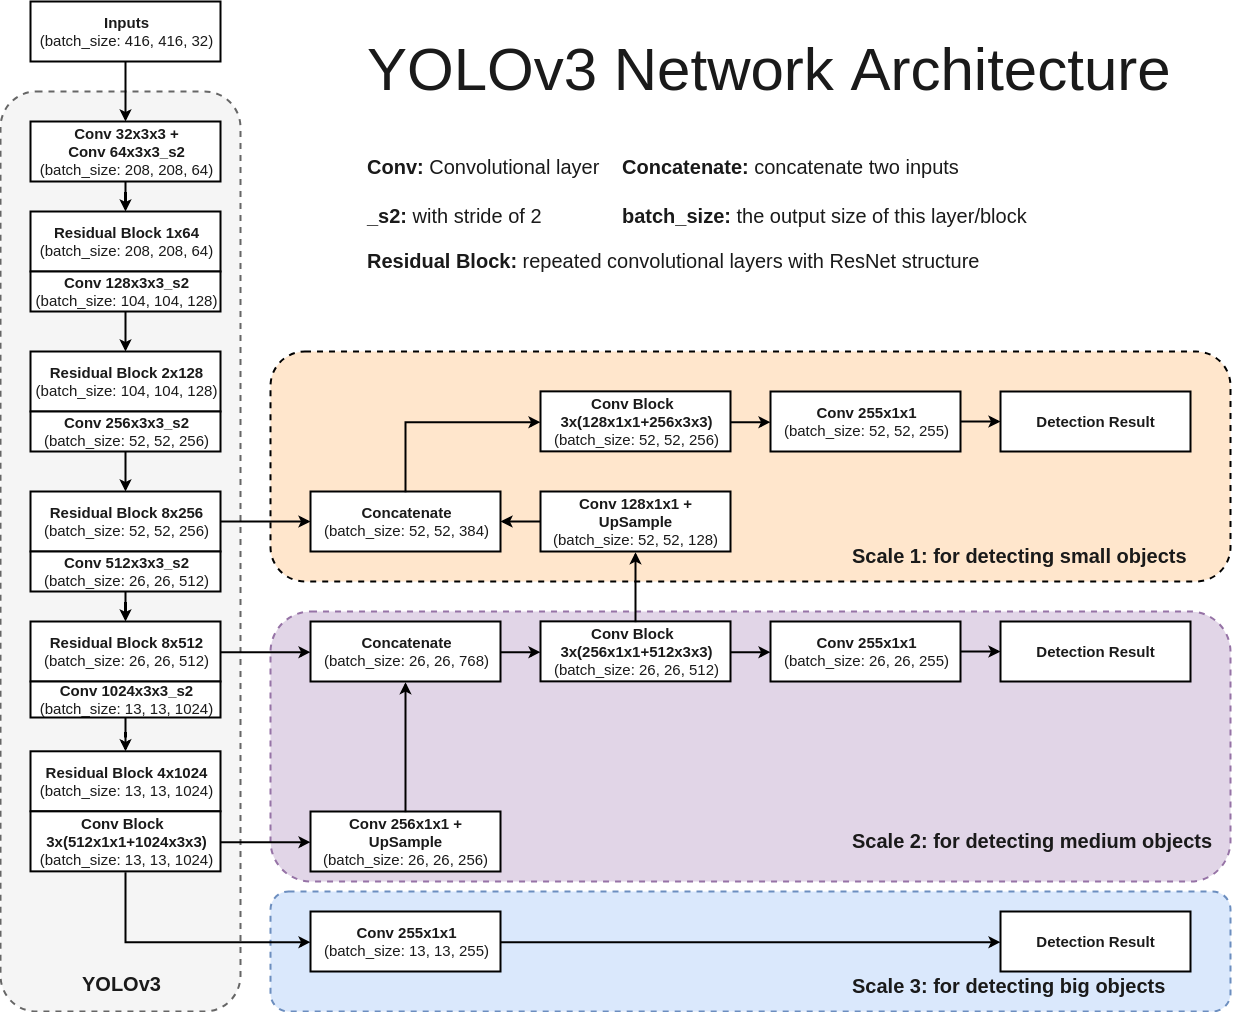
\includegraphics[width=\linewidth]{YOLOv3_architecture.png}
        \caption{Deep learning structure of Yolov3}
        \label{fig:yolov3}
    \end{figure}
    
    
    \begin{figure}[h!]
        \centering 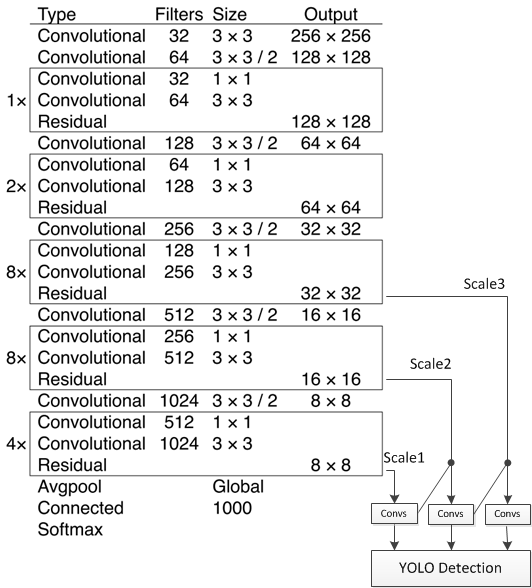
\includegraphics[width=0.6\linewidth]{lyy_YOLO_arch.png}
        \caption{High level diagram of Yolov3}
        \label{fig:yolov3_arch}
    \end{figure}

\paragraph{Realtime multi-person 2D pose estimation} Realtime multi-person 2D pose estimation is a key component in enabling machines to understand people in images and videos. It is a realtime method to detect the 2D pose of multiple people in an image. The proposed method uses a non-parametric representation, which is referred to as Part Affinity Fields (PAFs), to learn the association between body parts for individuals in the image. This bottom-up system achieves high accuracy and realtime performance, regardless of the number of people in an image. \cite{zhu2013pedestrian}
    
The architecture includes the following pipelines, which is also summarized in Fig. \ref{fig:openpose_arch}:

\begin{enumerate}
    \item First, the image is passed through a baseline network to extract feature maps. In the paper, the author uses the first 10 layers of VGG-19 model.
    \item Then, the feature maps are processed with multiple stages CNN to generate: 1) a set of Part Confidence Maps and 2) a set of Part Affinity Fields (PAFs) Part Confidence Maps is a set of 2D confidence maps S for body part locations. 
    \item Each joint location has a map. Part Affinity Fields (PAFs) are a set of 2D vector fields L which encodes the degree of association between parts.
    \item Finally, the Confidence Maps and Part Affinity Fields are processed by a greedy algorithm to obtain the poses for each person in the image.

\end{enumerate}

    \begin{figure}[h!]
        \centering 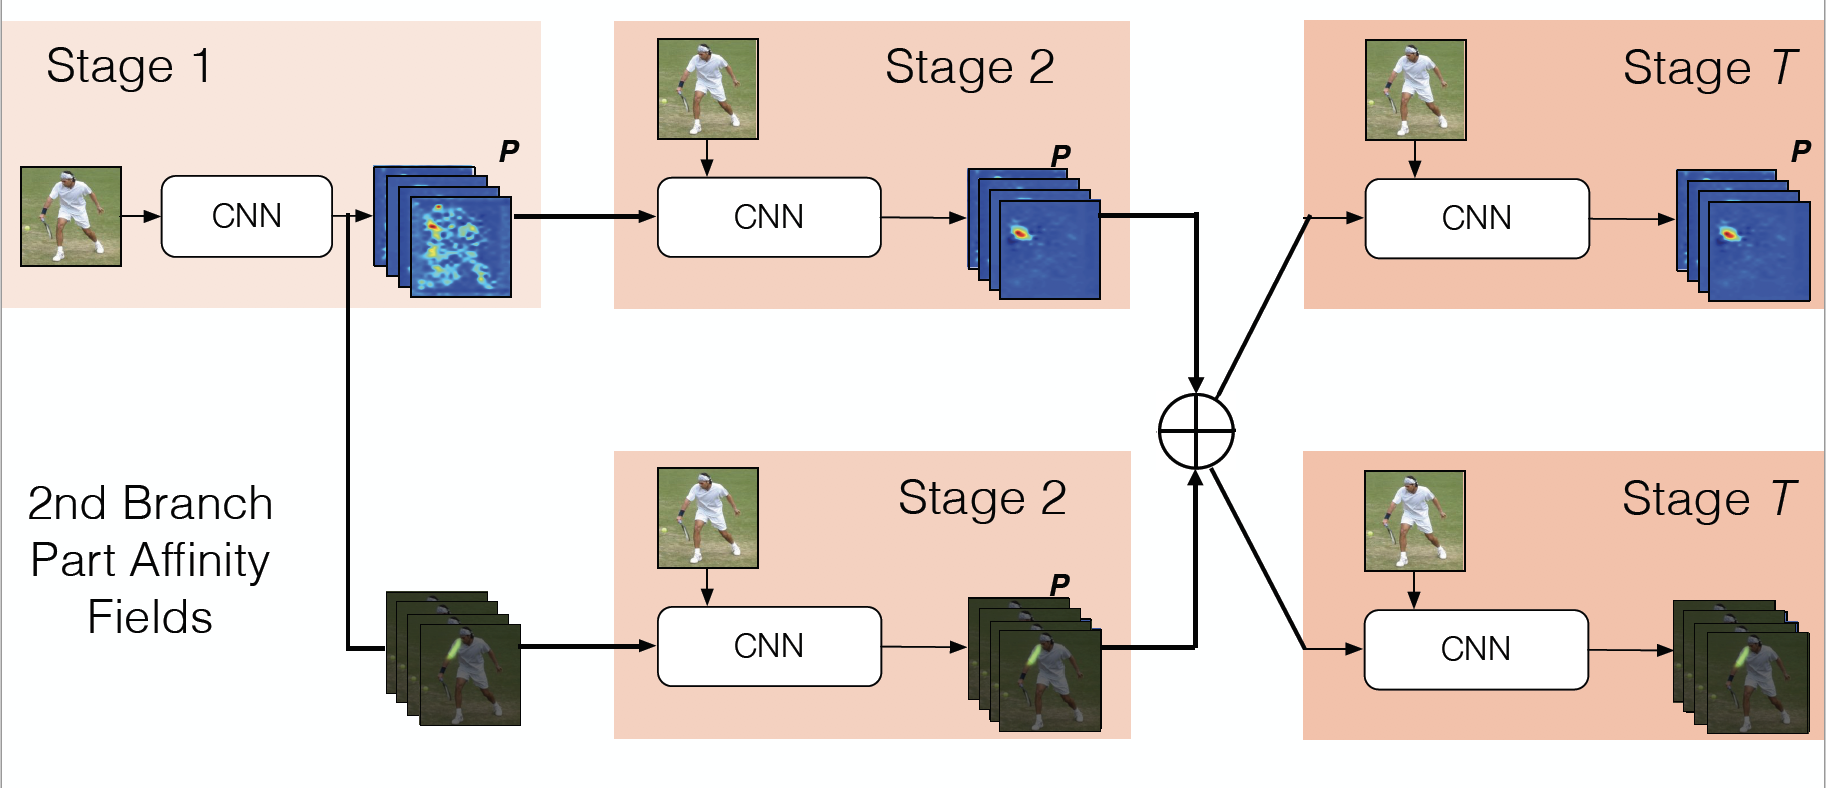
\includegraphics[width=0.6\linewidth]{lyy_OpenPose.png}
        \caption{High level diagram of OpenPose}
        \label{fig:openpose_arch}
    \end{figure}


\subsection{Manufacturing Plan}
% \yueying{Analog to the mechanical processes, describe detailed flow charts if the core of one project is about programming and simulation. Algorithms should still be explained in detail. Please list the programming language or software and the existing source codes or libraries you are going to use.
% }
For this project, we use Python3 as our programming language. Fig.\ref{fig:Manu_FlowChart} is the detailed flow chart of our project.
\begin{figure}[h!]
  \centering 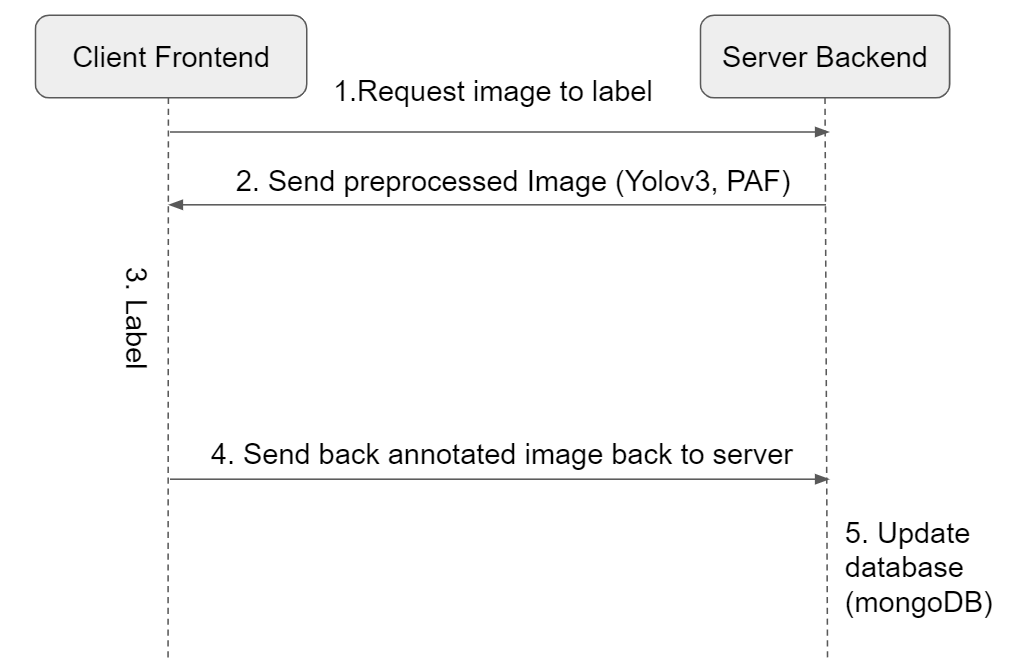
\includegraphics[width=\linewidth]{manufacture.png}
  \caption{Manufacturing Flow Chart}
  \label{fig:Manu_FlowChart}
\end{figure}

For step 1 and step 4, we use Flask as our framework and REST API to handle the communication between client and server. 

For step 2, server backend will preprocess the image using our deep learning model. The detailed algorithms here are Yolov3 for object detection and PAF for human pose estimation.  


For step 3, we use PyQt5 as our library to customize the open sourcing project Labelme. 

After users send back their labeled images to the server, in step 5, server uses mongoDB as database to manage the status of image set.

To sum up, in our project, the existing source codes are:
\begin{itemize}
    \item Labelme\cite{labelme}, YOLOv3\cite{Redmon2018YOLOv3}, Openpose\cite{Cao2016Realtime}
\end{itemize}
The packages we have used are 
\begin{enumerate}
    \item \textbf{Preprocessing} 
    \begin{itemize}
        \item     'matplotlib>=3.1',
         \item 'numpy>=1.16',
        \item  'Pillow>=2.8',
        \item  'PyYAML>=5.1',
    \item 'qtpy>=1.8',
    \item 'termcolor',
    \item 'jsonpickle>=1.2',
    \item 'scipy>=1.2',
     \item 'configobj',
     \item 'keras',
     \item 'tensorflow>=1.8,<2',
     \item 'sip',
     \item 'pyqt5>=5.12',
     \item 'opencv-python',
     \item 'IPython'
       \end{itemize}
    \item \textbf{GUI}
    \begin{itemize}
        \item QtPy
    \end{itemize}
\end{enumerate}
  


\subsection{Validation Plan}
There are three important criteria in our engineering specifications: accuracy (correct rate of annotation) in preprocessing, coverage (ratio of annotated objects to total objects) in preprocessing and annotation efficiency. 
We plan to test the previous two criteria by going through the annotation process with our software, and a test suit of 100 images is provided by the sponsor. We manually calculate the average accuracy and coverage in proprocessing for the test suit.\\
For the annotation efficiency, since it is very subjective and should be done by people new to our software, the company will have a group of people using our software and giving us feedback about their user experience of our product comparing with others. We will base our assessment on their feedback and do several iterations to improve efficiency if necessary.